\chapter{Experiment 3: Relearning a task}
\label{exp3}
The motivation behind reusing modules is as mentioned in the introduction, to increase the number of tasks a PathNet can learn before being saturated by decreasing the amount of new capacity a path needs for a new task. A optimal search algorithm for new paths should therefore be able to reuse as much knowledge as possible without limiting the performance. If we assume a ideal search algorithm would find optimal modules for each task, it should be able to find and reuse all learned knowledge if a task is learned twice. 

We can put this to the test by learning some task twice for all seven algorithms in chapter \ref{exp2}. As the amount of module reuse in these experiments were small, we lower the proverbial bar here by reducing the module search space.

The question we want to answer is this: \textit{"Given optimal conditions for module reuse\footnote{By optimal conditions we mean learning a task where a full set of parameters is already optimized for that task.}, which selection pressure scheme is best suited for knowledge reuse?"}

\section{Description}
The experimental structure here is simple. The same experimental parameters as the experiment in chapter \ref{exp2} are used again, but here the the seven algorithms will here be applied to a binary task problem where both tasks are the same: a cSVHN classification problem with all 10 classes. After searching for a optimal path for both tasks, the reuse is noted. 

By performing this experimental trial for each algorithm multiple times, we can compare the observations of reuse with the probability of seeing these results in random module selection, and then with each other. 

\section{Hypothesis}
Based on the reuse in the previous selection pressure experiments, we do not expect any algorithm to yield perfect results\footnote{Perfect results here would constitute finding all modules used in the previous path}, but instead have a statistically significant difference from random module selection. Given the algorithms different selection pressures, they are expected to give somewhat different reuse results.

As each search should be capable of reaching a decent validation accuracy on its own, it is not expected that there will be a significant difference between task 1 and task 2 for any of the algorithms. However, there is no reason to believe the effects the different tournament sizes have on accuracy will be any different than in chapter \ref{exp2}. 

\section{Experimental setup}
The experiment structure here is a binary task problem, where we want to find two paths for a full cSVHN classification problem twice, meaning both task 1 and task 2 is cSVHN classification with all classes. The two searches should have a non-zero probability of zero reuse, so the PathNet dimensions are set to 3 layers of 6 modules each with a maximum of 3 active modules pr. paths layer. We can describe the total number of possible paths as 
\begin{equation*}
    \prod_{i=0}^{\omega-1}(M-i)^{L}
\end{equation*}
where \(\omega\) is the maximum number of active modules in each layer for each path, \(M\) is the number of modules in each PathNet layer and  \(L\) is the number of layers in the PathNet. This means the number of possible paths in a 20-by-3 PathNet with \(\omega=3\) is  
\begin{equation*}
    \prod_{i=0}^{3-1}(20-i)^{3}\approx 3.2\times10^{11}
\end{equation*}
and in this experiment
\begin{equation*}
    \prod_{i=0}^{3-1}(6-i)^{3}\approx 1.7\times10^{6}
\end{equation*}
Reducing the PathNet size from 20 modules in each layer to 6 have reduced the search space with 5 orders of magnitude, and it should therefore be significantly easier to find reusable modules here than in the previous experiment.

\begin{table}[ht]
    \centering
    \begin{tabular}{clll}
    \# of reuse & \# of outcomes & Monte-Carlo probabilities & Rounded  \\
    0           & 88892859      & 0,088892859               & 0,0888928 \(\pm 10^{-7}\)  \\
    1           & 266671854     & 0,266671854               & 0,2666718 \(\pm 10^{-7}\)  \\
    2           & 327560805     & 0,327560805               & 0,3275608                  \\
    3           & 213925123     & 0,213925123               & 0,2139251                  \\
    4           & 81393230      & 0,08139323                & 0,0813932                  \\
    5           & 18720470      & 0,01872047                & 0,0187205                  \\
    6           & 2612531       & 0,002612531               & 0,0026125                  \\
    7           & 213747        & 0,000213747               & 0,0002137 \(\pm 10^{-7}\)  \\
    8           & 9195          & 0,000009195               & 0,0000092                  \\
    9           & 186           & 0,000000186               & 0,0000002                 
    \end{tabular}
    \caption{Results from Monte-Carlo approximation of reuse probabilities for two paths in a 6-by-3 PathNet with a maximum of 3 active modules in each layer.}
    \label{tab:montecarlo}
\end{table}

We can approximate the probability of finding any number of reuse by randomly selecting two paths within the limitations of the PathNet dimensions and path-size with a Monte-Carlo approach. Using equation \ref{eq:montecarloP} where we want the probabilities to be minimum 10 times as large as the standard deviation (\(R=0.1\)) and \(n=10^{9}\) Monte-Carlo trials, we calculate the probability accuracy to be 
\begin{equation*}
    \frac{1}{nR^{2}+1}=\frac{1}{10^{7}+1}\approx10^{-7}
\end{equation*}
Meaning we can tell the probability of reuse to the seventh decimal place from the Monte-Carlo results. The results of the performed Monte-Carlo estimation can be found in table \ref{tab:montecarlo}.

We will calculate the expected reuse distribution based on the Monte-Carlo estimated probabilities, and use Mann-Whitney tests to see how the algorithms reuse holds up compared to expectations. 

Learning from the conclusion in chapter \ref{exp2}, the algorithms maximum tournament size is reduced from 25 to 10.

\section{Results}

\subsection{Population Diversity}
\begin{figure}[h!]
    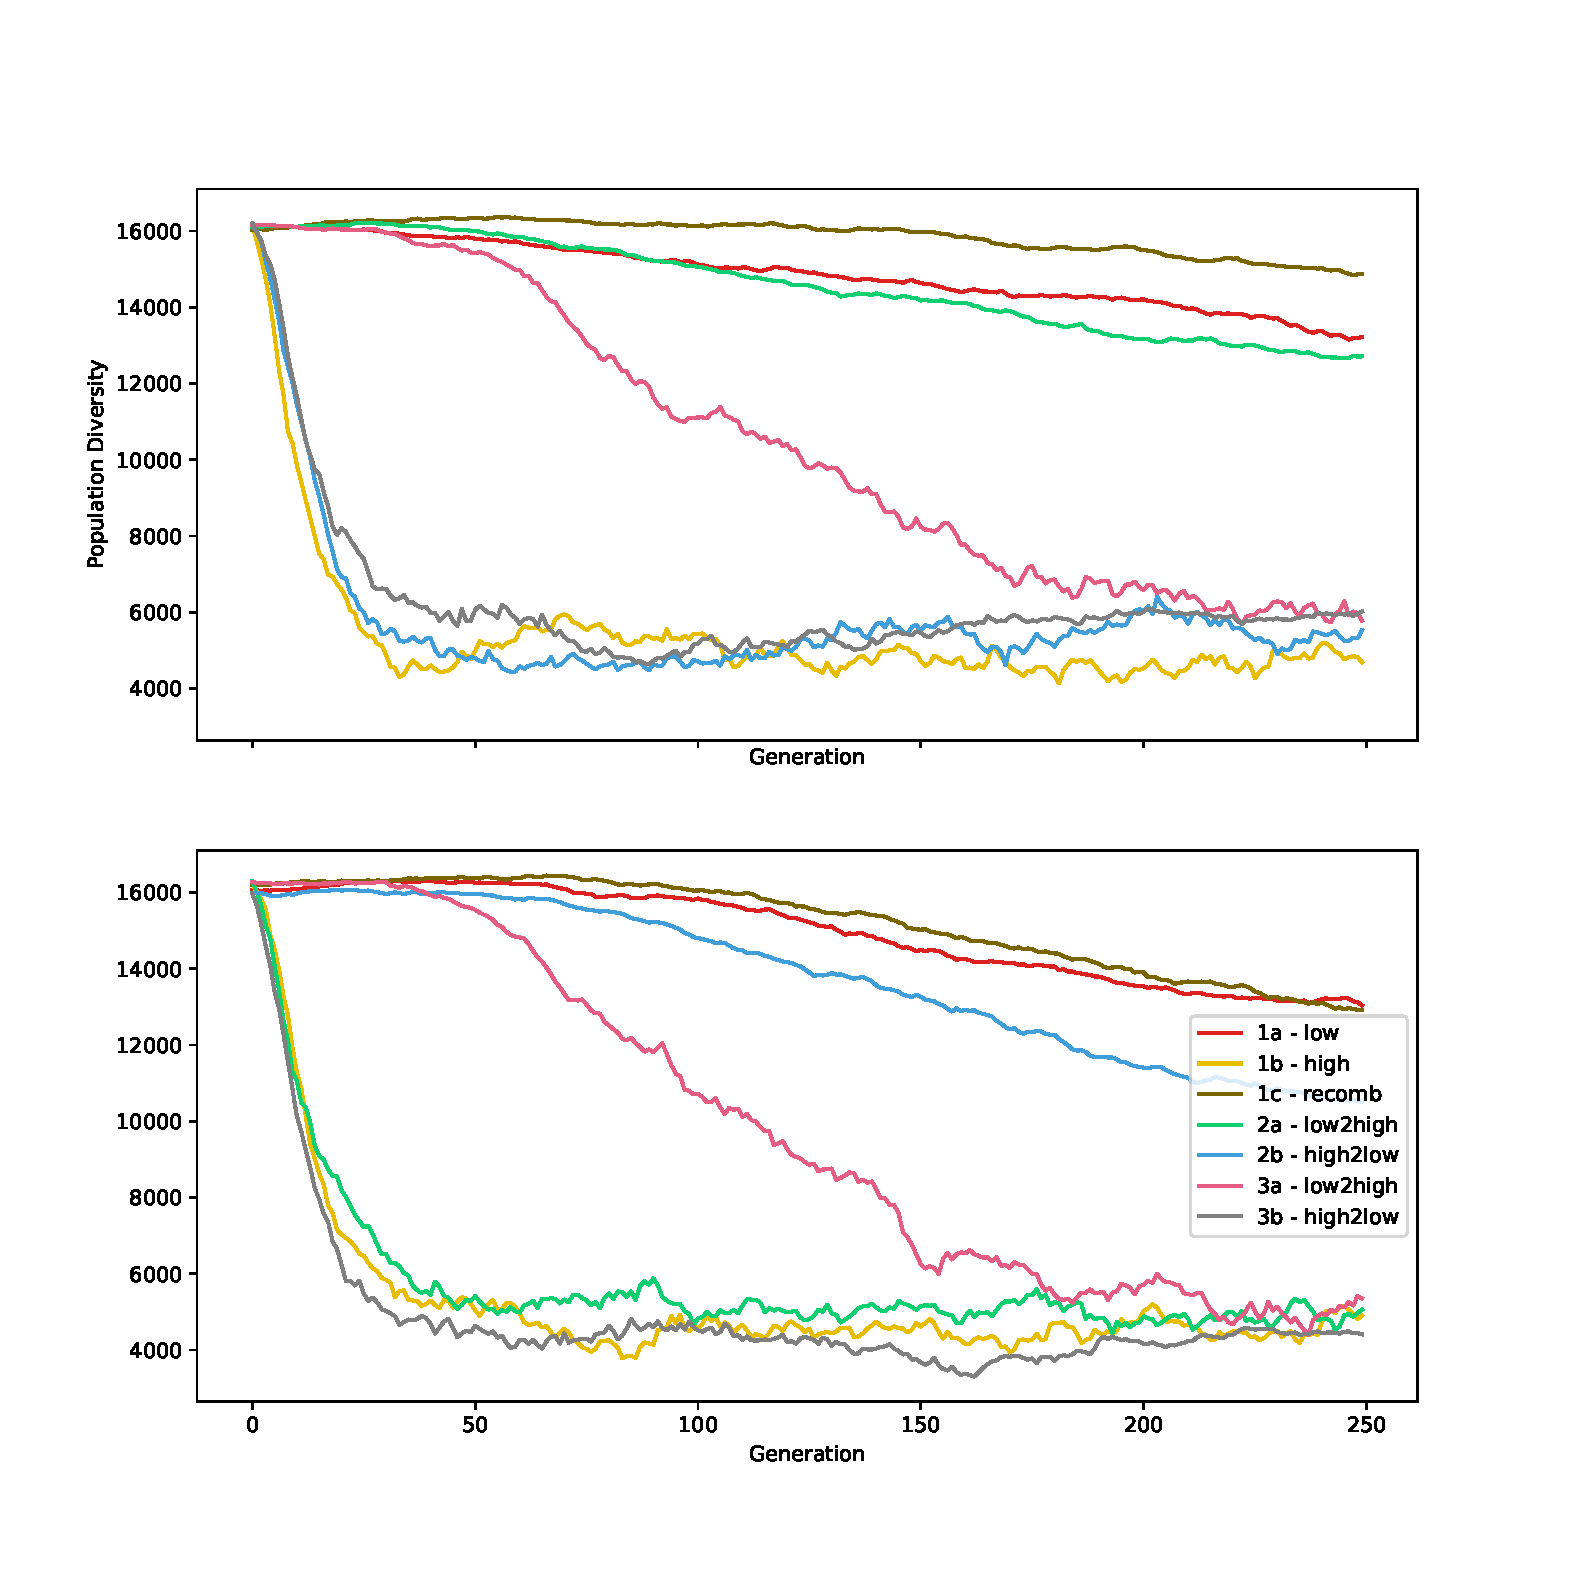
\includegraphics[width=\textwidth, center]{Chapters/4.Experiments/exp3/figures/diversity_hamming.pdf}
    \caption[Hamming diversity plot]{The average pair-wise Hamming distance diversity for each algorithm over 250 generations.}
    \label{fig:exp3.hamming}
\end{figure}
\begin{figure}[h!]
    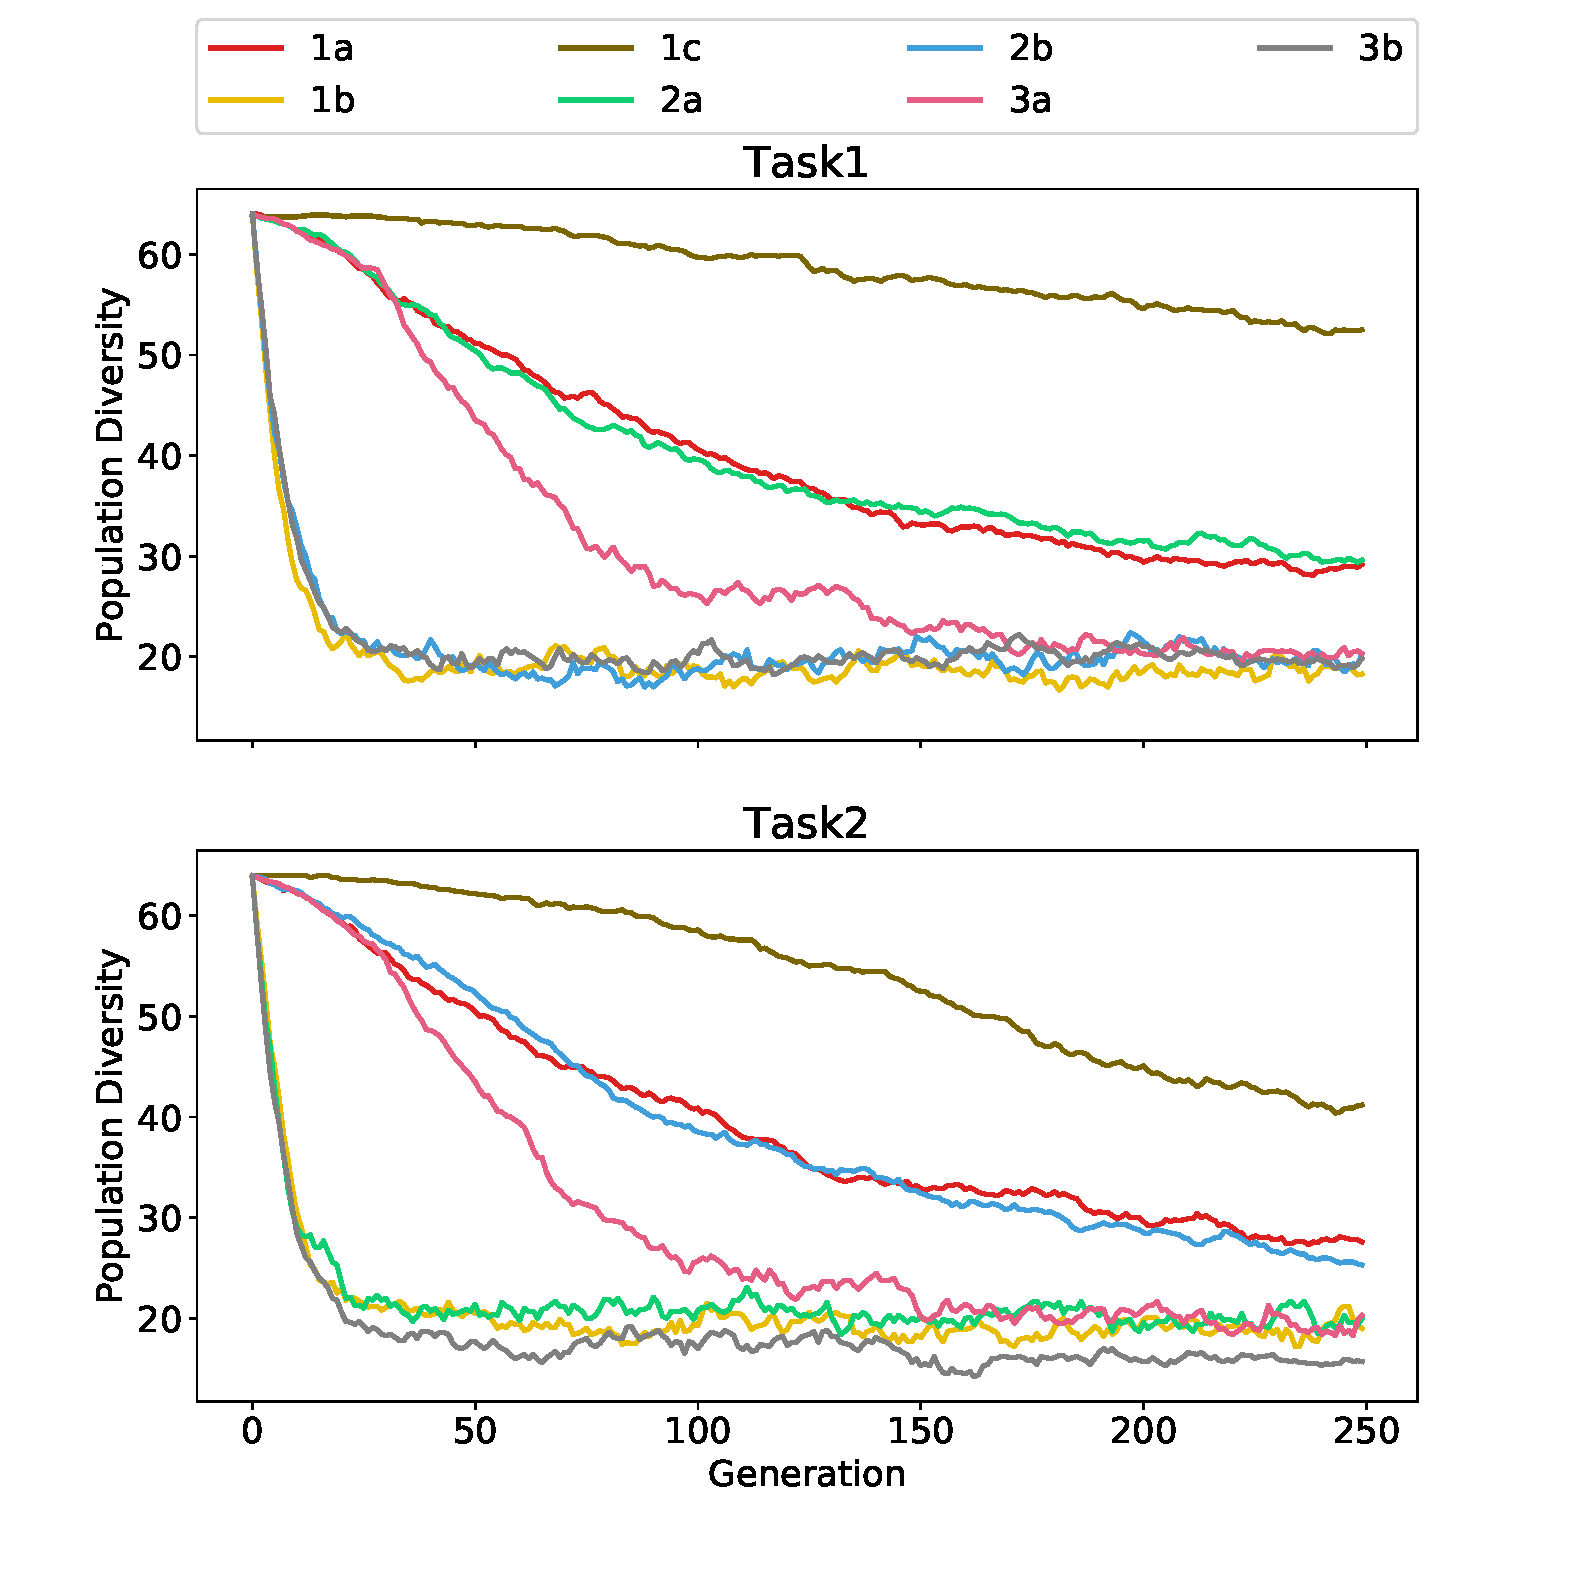
\includegraphics[width=\textwidth, center]{Chapters/4.Experiments/exp3/figures/diversity_frequency.pdf}
    \caption[Frequency diversity plot]{The average amount of unique paths for each algorithm over 250 generations.}
    \label{fig:exp3.frequency}
\end{figure}

As the algorithms that run here are the same as in chapter \ref{exp2}, the convergence rates are quite similar to figures \ref{fig:exp3.hamming} and \ref{fig:exp3:frequency}. However, the searches are run for 250 generations, which makes the diversity drop in algorithms with slow convergence, such as 1a and 1c, become apparent. 

Noteworthy about these diversity plots is that algorithm 1c in both cases converge more within the 250 generations for task 2 than task 1. Testing the null-hypothesis that the final generations population have a similar pair-wise Hamming distance for task 1 than task 2 gives a p-value of 0.00229 for a one-sided Mann-Whitney test. Confirming the observation is not due to a outlier in the data, but rather a difference in the diversity distributions. The only other algorithms that change their convergence between task 1 and task 2 are algorithms 2a and 2b for obvious reasons.  

\subsection{Modular reuse}
\begin{sidewaysfigure}[p!]
    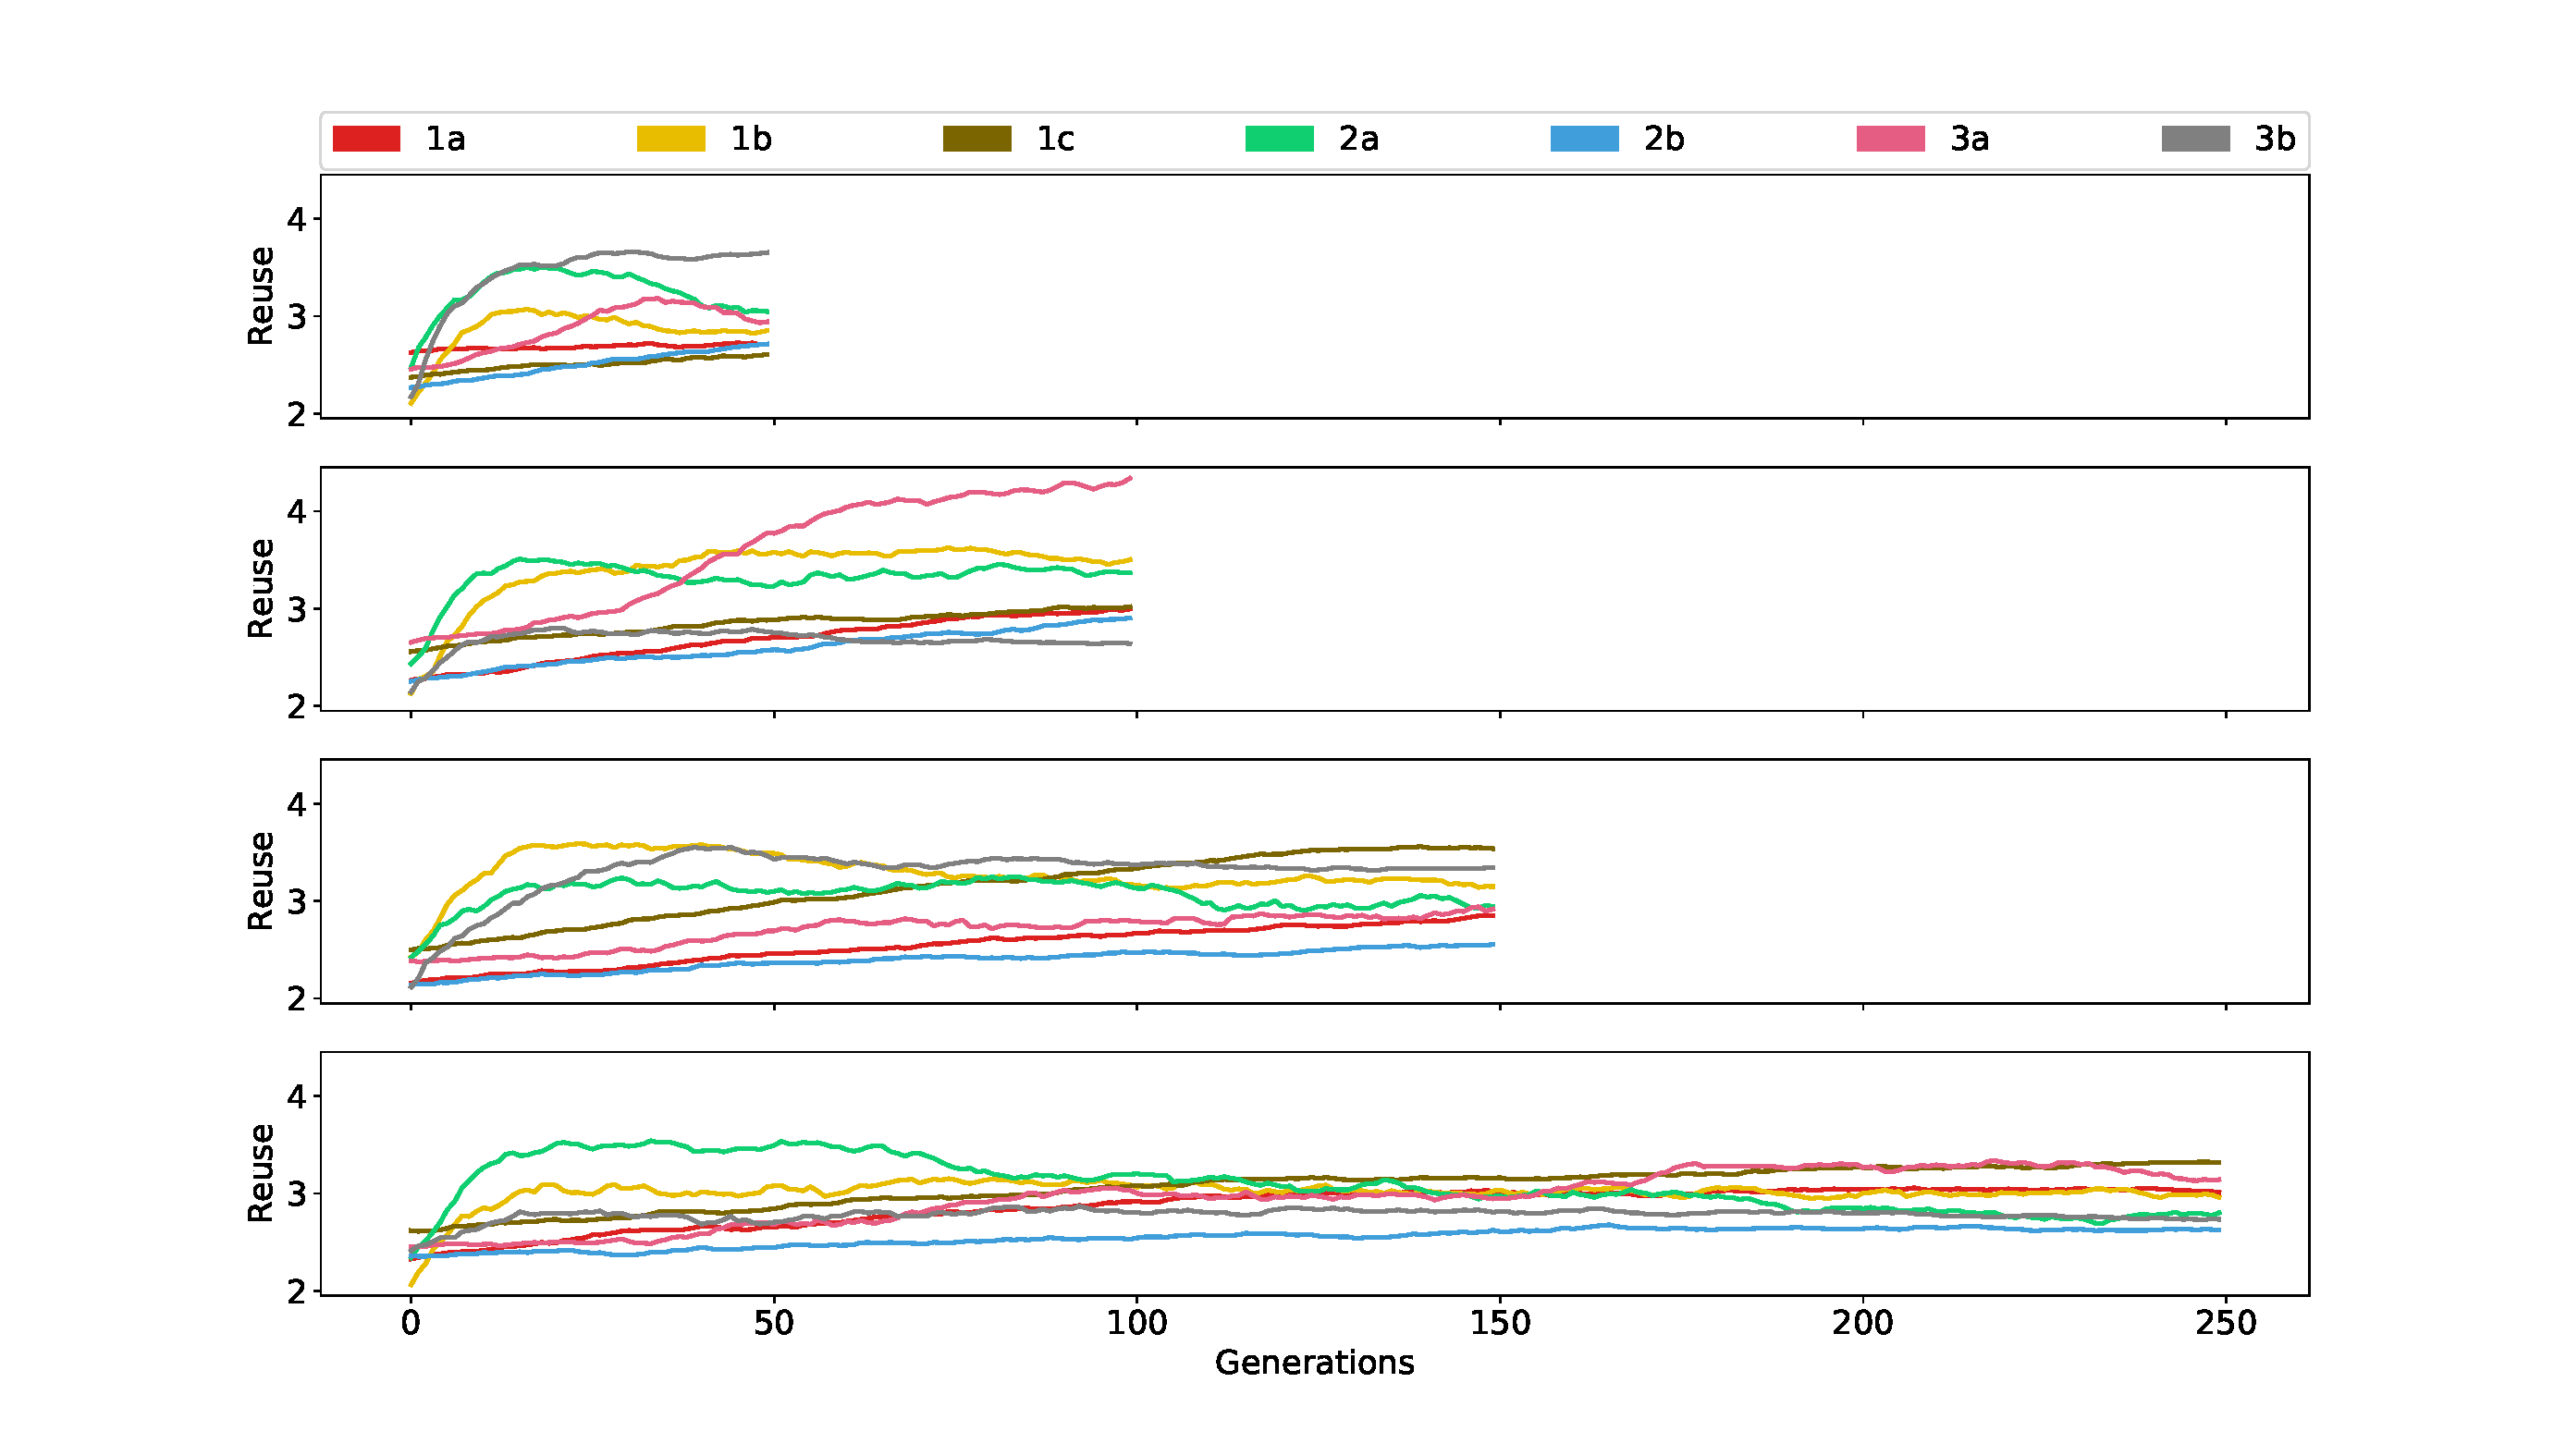
\includegraphics[width=1.2\textwidth, center]{Chapters/4.Experiments/exp3/figures/reuse_progression.pdf}
    \caption[Module reuse during search]{The change in reuse plotted over the search duration. Four generation limits were used, but the reuse during search are expected to be the same across the different search termination limits.}
    \label{fig:exp3.reuseprogression}
\end{sidewaysfigure}
\begin{figure}[h]
    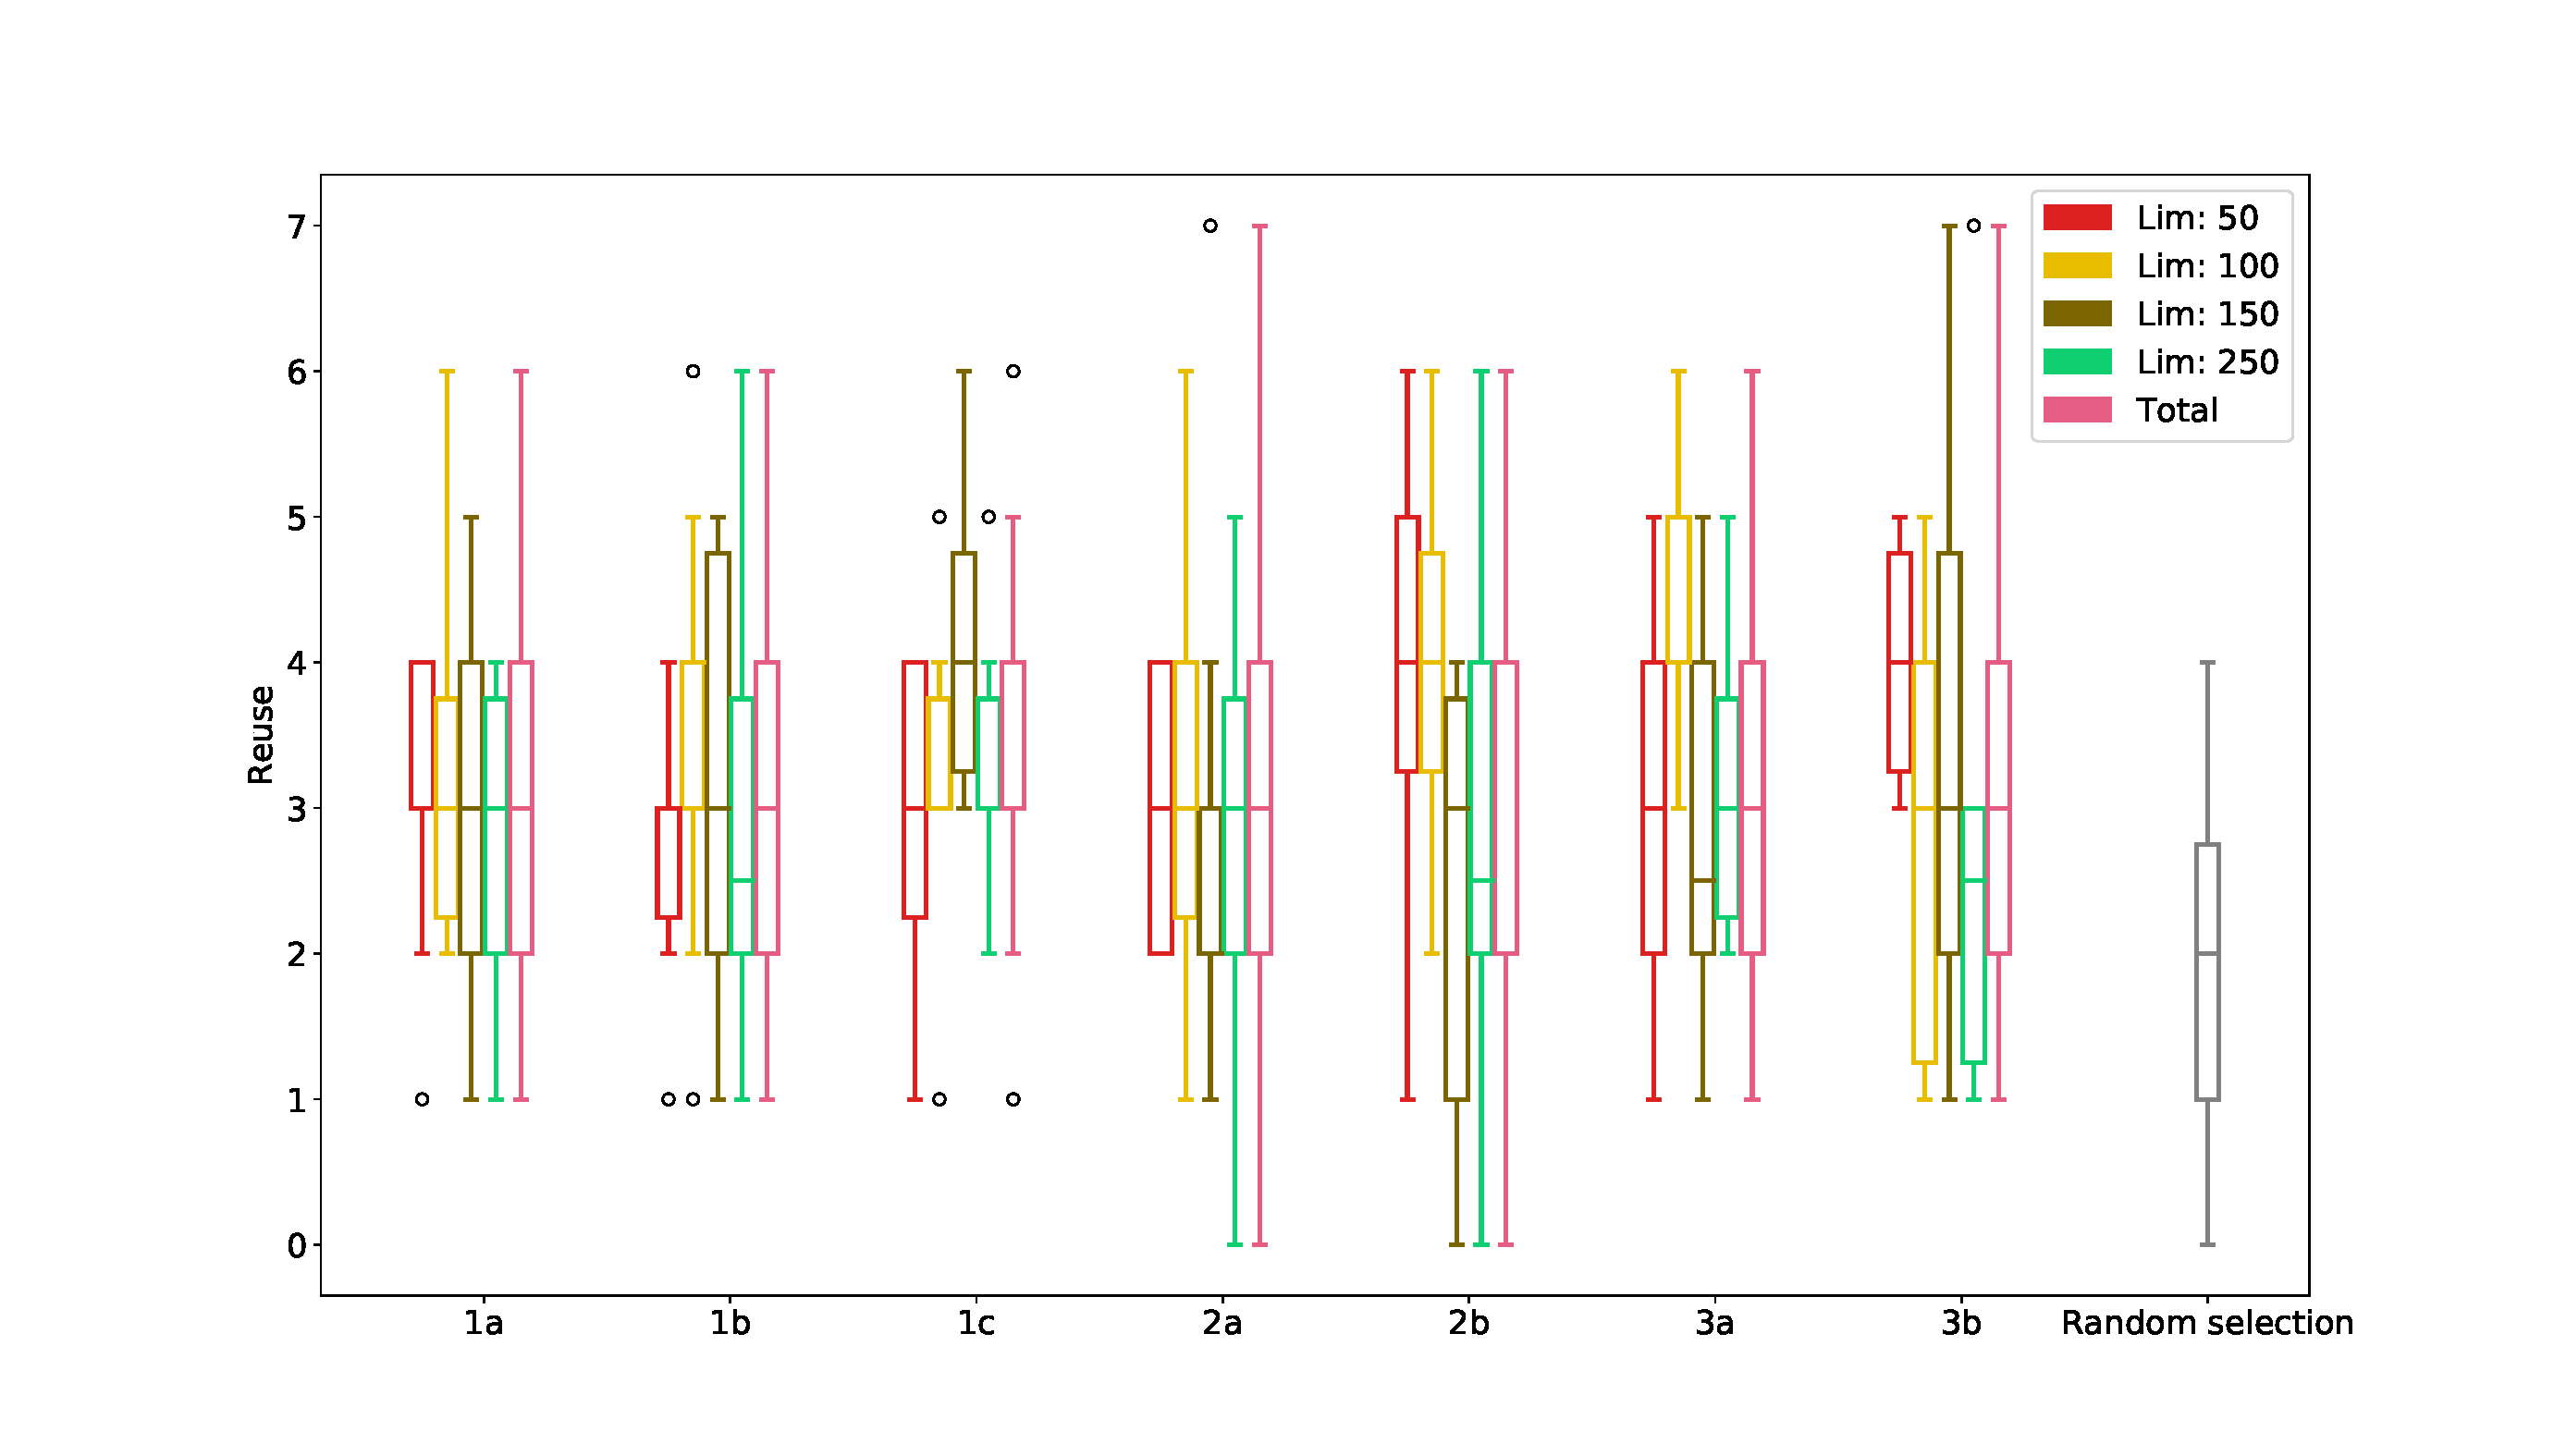
\includegraphics[width=1.25\textwidth, center]{Chapters/4.Experiments/exp3/figures/reuse_boxplot.pdf}
    \caption[Module reuse boxplot]{The average amount of unique paths for each algorithm over 250 generations.}
    \label{fig:exp3.reuseboxplot}
\end{figure}

Figure \ref{fig:exp3.reuseprogression} show the average reuse for each algorithm changing during the searches with different termination limit. Algorithms with high reuse for the second task (1b and 2b) reach the highest level of reuse within the first 30 generations, whereupon it start to drop. Algorithms using a low tournament size instead gradually increase in reuse, where it looks to surpass the other algorithms around 100 generations.  

The box-plot in figure \ref{fig:exp3.reuseboxplot} show the reuse in the optimal paths selected for task 2. The searches are stopped at different points, but there does not look to be any striking differences in any of the groups of reuse. They do all, however, seem to score higher than the expected reuse from random modules selection. 

When performing MWW testing to compare the algorithm results to that of random module selection, we do not want to run multiple test like in chapter \ref{exp2}, as the Bonferroni correction to the \(\alpha\) level would most likely cause none of the null-hypotheses to be rejected due to the number of tests we need to perform. Instead MWW-test where the reuse groups for each algorithm is added together are compared to the estimated reuse for such a group if modules were selected randomly. The p-values for all four generation limit are on the order of \(10^{-4}\) which makes all the null-hypotheses rejected and the difference significant. 

Another set of MWW-tests were run to check the difference in reuse for the different generation limits. These tests concluded with the only significant difference between generation limits being that of 250 and 100, where a generation limit of 100 generations gave a significantly higher distribution of module reuse. A full table of the p-values can be found in table \ref{tab:ptable.generationlimit}.

\subsection{Path fitness}
\begin{sidewaysfigure}[h]
    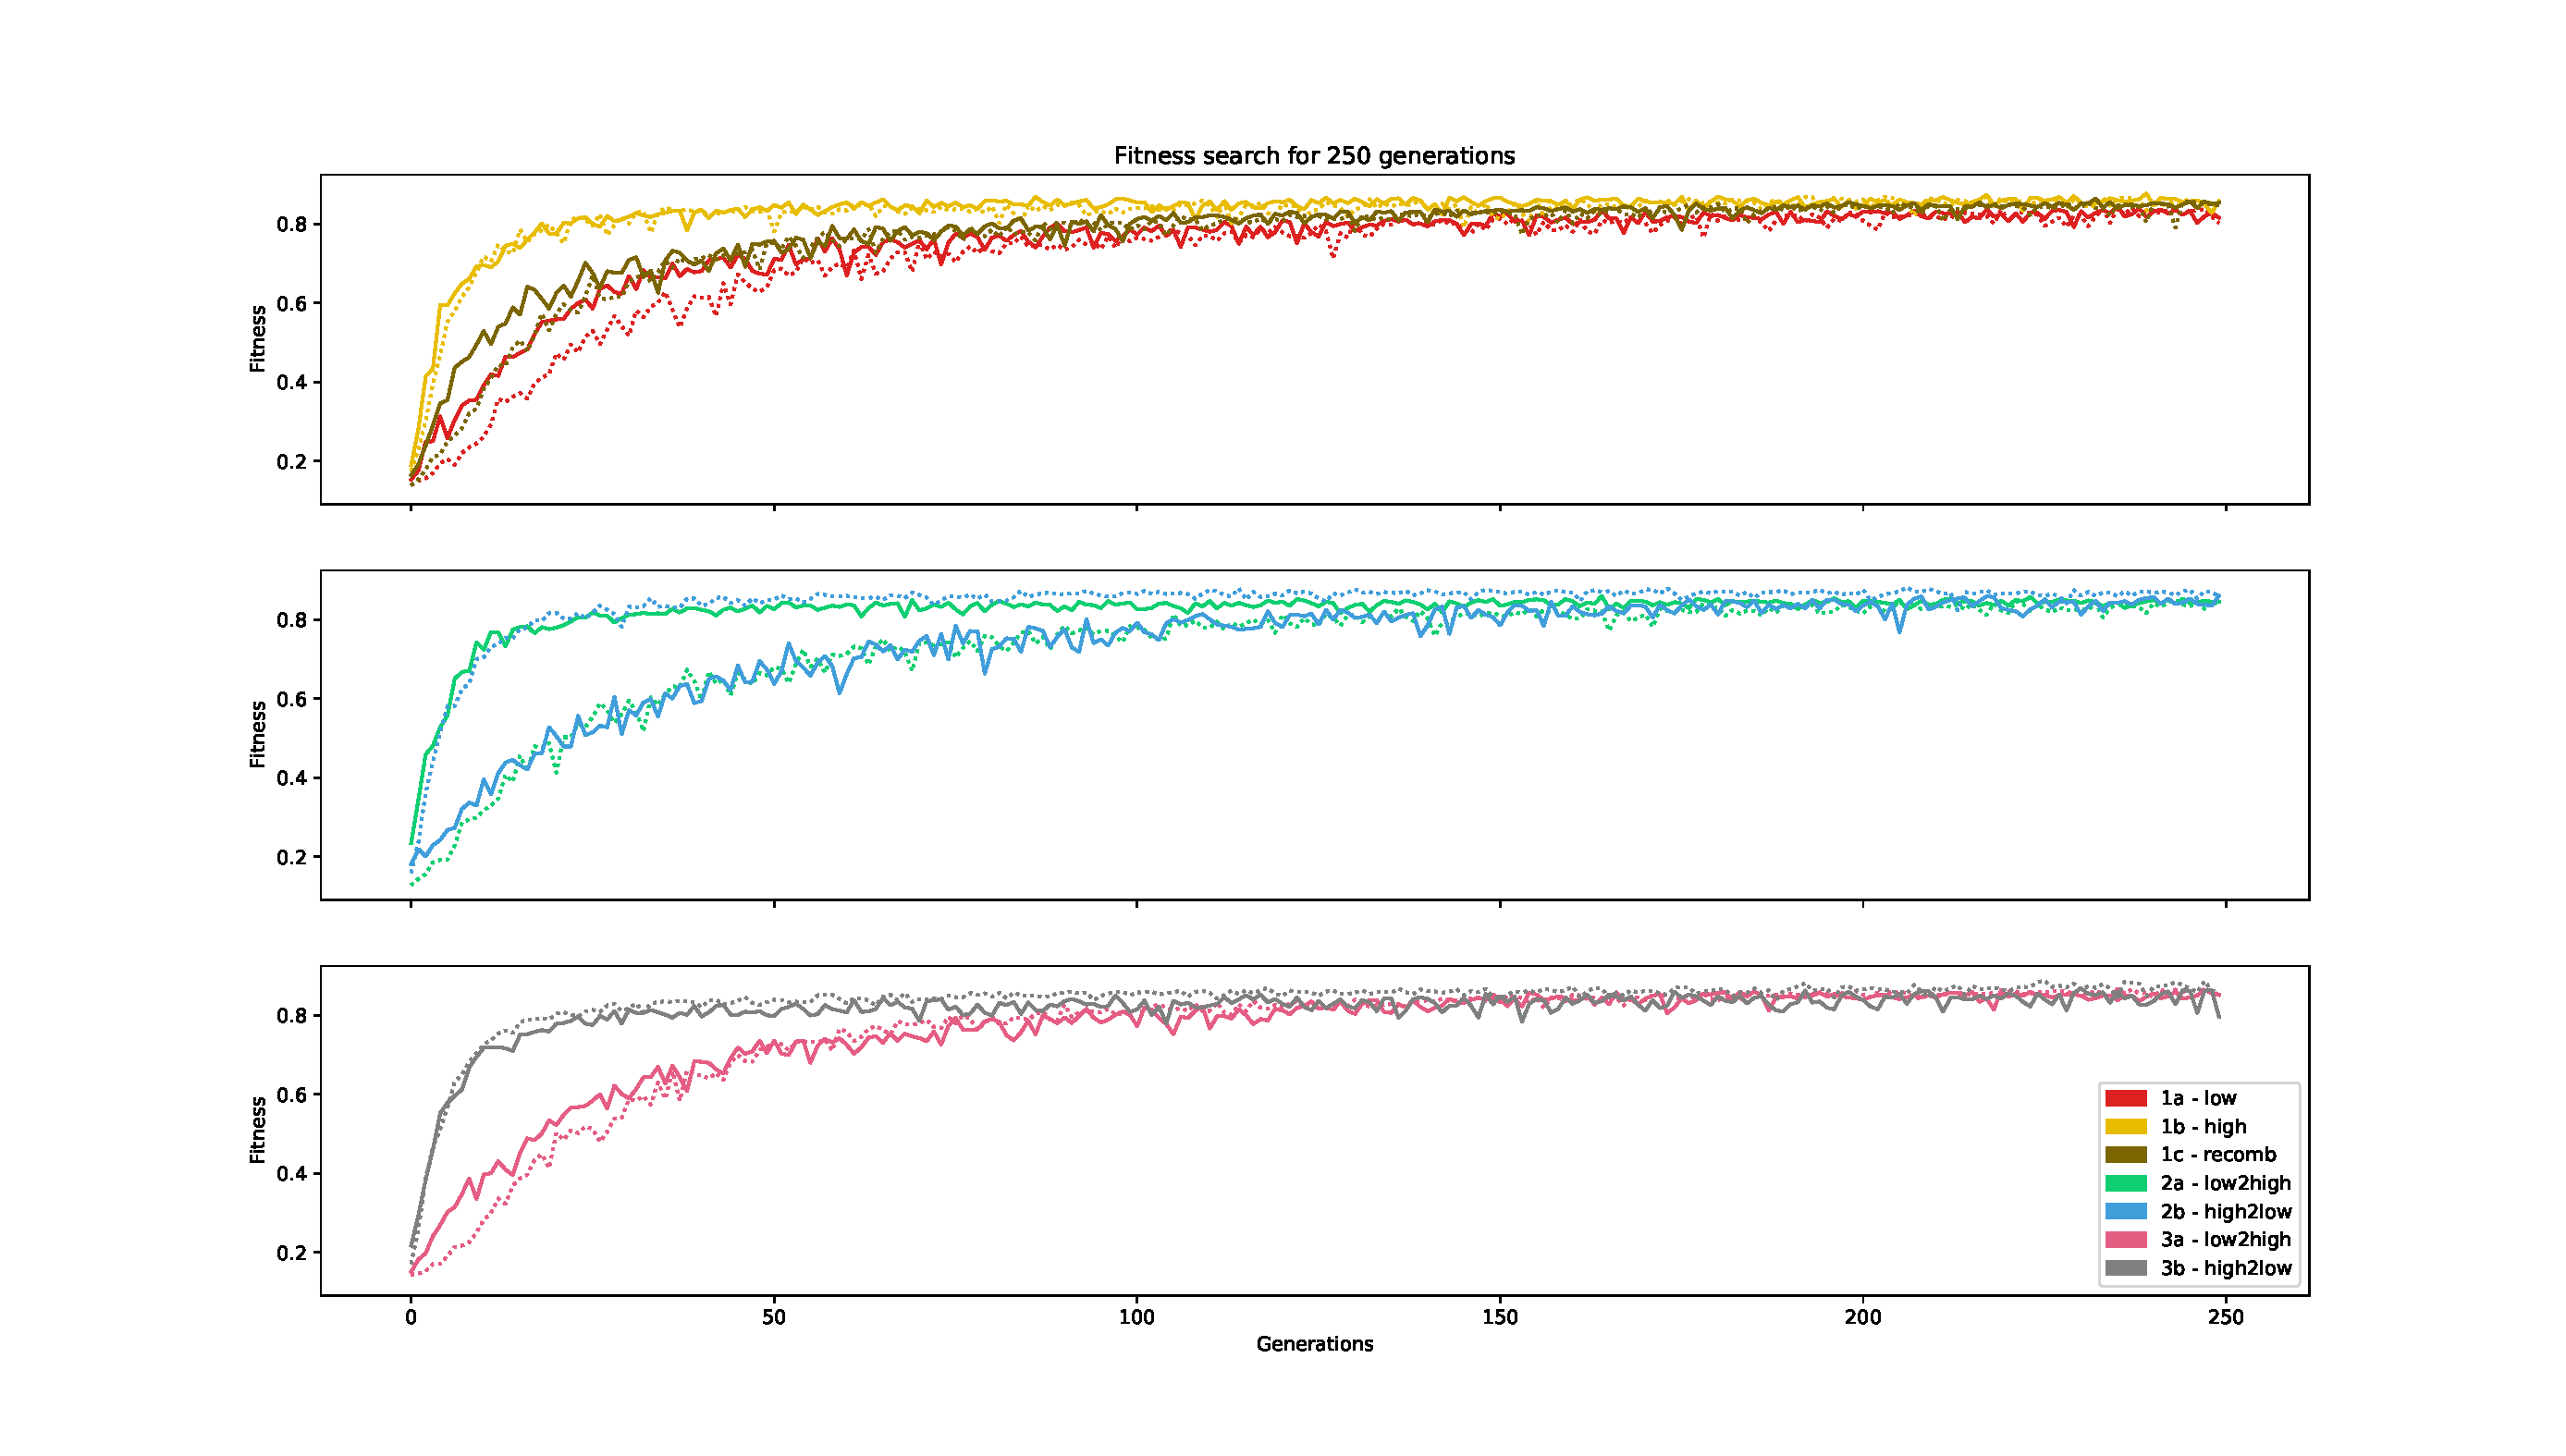
\includegraphics[width=1.25\textwidth, center]{Chapters/4.Experiments/exp3/figures/fitness_progression.pdf}
    \caption[Changes in average tournament fitness]{The average tournament fitness for each generation. The dotted lines are average fitness during search for task 1, while the whole lines are for task 2.}
    \label{fig:exp3.fitness}
\end{sidewaysfigure}

\begin{sidewaysfigure}[h]
    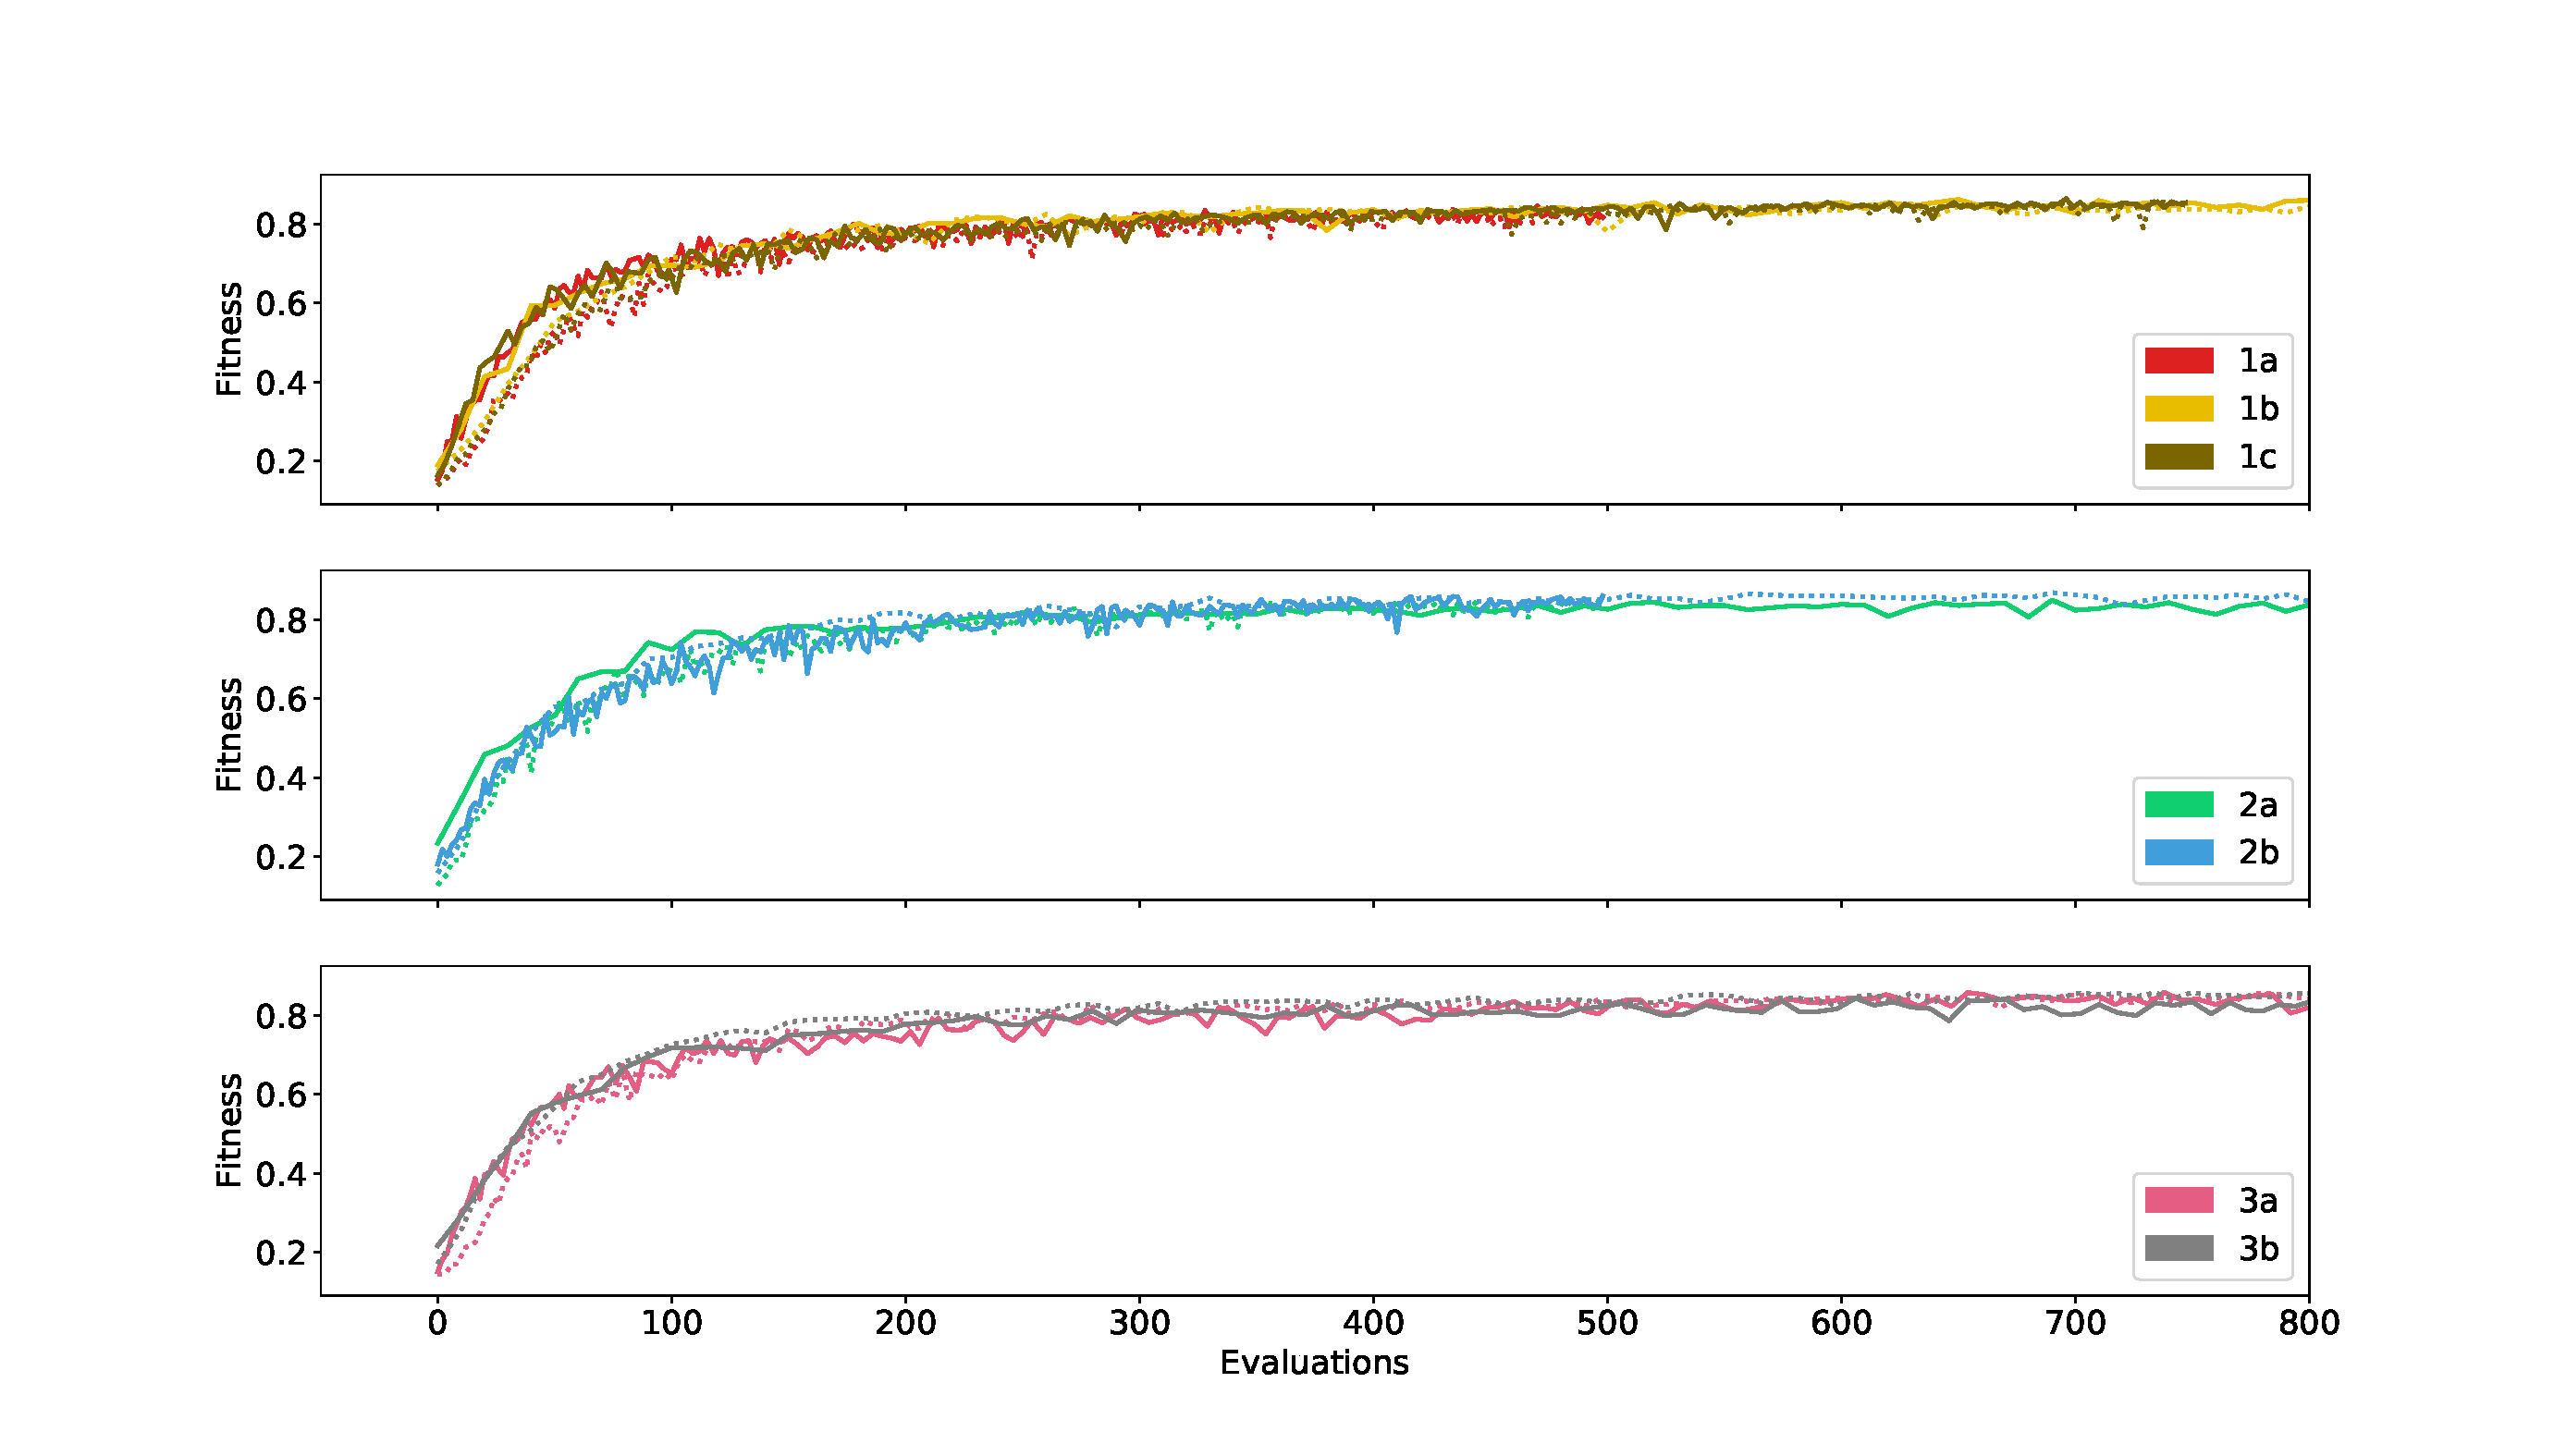
\includegraphics[width=1.25\textwidth, center]{Chapters/4.Experiments/exp3/figures/fitness_by_evaluations.pdf}
    \caption[Average tournament fitness plotted by evaluation]{The average tournament fitness as it changes with respect to number of evaluations for the first 800 evaluations.}
    \label{fig:exp3.fitness_by_evaluations}
\end{sidewaysfigure}

Figure \ref{fig:exp3.fitness} show the average tournament fitness for each generation. As with results in chapter \ref{exp2}, the algorithms with high tournament size plateau in fitness quicker than algorithms with a low tournament size.

Noteworthy features of this plot are the increase in average fitness for algorithms with low tournament size in the start of each search from task 1 to task 2, suggesting the learning for these algorithms are easier the second time around. 

The plot in figure \ref{fig:exp3.fitness_by_evaluations} show the same progress in average tournament fitness, but here plotted by evaluation number and not generation. This figure shows us the increase in average fitness from task 1 to task 2 is not only for the low tournament size algorithms. 

\section{Discussion}
As we expected from these relearning experiments, the level of modular reuse between tasks were higher than in chapter \ref{exp2}. Some of the increase is due to the smaller PathNet structure and permutation-space of modules, but as the MWW-tests for algorithm groups in figure \ref{fig:exp3.reuseboxplot} showed, the reuse these algorithms caused are significantly higher than that caused by random module selection. This tells us there are some incentive to reuse knowledge from task 1 in task 2.

Due to the different convergence rates, the reuse was expected to have different distributions for the different generation limits. The MWW-tests and p-values in table \ref{tab:ptable.generationlimit} shows us this is true for the searches limited at 250 and 100 where there shorter search time yielded more reuse. 

The only difference between task 1 and task 2 is that task 2 searches among modules where some contain with pre-trained parameters. The figures \ref{fig:exp3.fitness} and \ref{fig:exp3.fitness_by_evaluations} confirm then that reusing locked modules improves training as the average fitness of a tournament grows quicker for task 2. One can only assume this effect would get more prominent for a more complex task-domain where generalization is difficult and reusing knowledge becomes more valuable.   

\section{Conclusion}
These experiments did not provide any conclusive evidence for which selection pressure scheme that optimized module reuse, as there were not shown any difference between the algorithms. However, as hypothesized, they did reach a higher module reuse than that of a random module selection. 

The paths that had some knowledge to reuse did perform better than those who optimized newly trained parameters. This confirms the benefit to PathNet is present also here. 